% Chapter 4 from the standard thesis template
% that contains an adv. example table and figure.
\chapter{SOFTWARE DEFINED RADIOMETER IMPLEMENTATION}\label{ch:implementation}

One of the principal goals with this research was to implement a fully functioning total power radiometer within software.  The N200 provides us the link between the RF signal captured by the antenna and converts that to a format that can now be used by the to manipulate the signal.  Once the signal has been passed to the computer, GNURadio will implement the correct algorithms to detect the power within the signal, filter and output the information.  

One of the advantages of course with a SDR is that filtering can also be done within the software.  In addition, thanks to the WxGUI that GNURadio uses, we can also build a user interface that can control several key variables that are useful for us.  This includes controlling the gain on the programmable gain amplifier on the DBSRX2 card, the sampling or bandwidth of the signal, the center frequency, and also the integration time.  All of these can now be controlled in real time as well.  GNURadio will also store the power data so that we are able to do further analysis of the data using a software program like Matlab or Python.  Because GNURadio is a very flexible system we are able to do more with the signal such as filtering, polarimetric  radiometer, and frequency analysis.  We are also able to add additional features and improvements through updates to the software.

\section{Requirements}

To help us quantify the required performance of the radiometer, information was provided to us by Dr. Brian Hornbuckle and also derived from existing radiometers.  The requirements given are outlined in table \ref{rad_performance}.

\begin{table}[h!tb] \centering
\isucaption{Required Radiometer performance}
\label{rad_performance}
% Use: \begin{tabular{|lcc|} to put table in a box
\begin{tabular}{lcc} \hline
\textbf{Parameter} & \textbf{Value} & \textbf{Units} \\ \hline
Minimum bandwidth & 20 & MHz \\
Operational frequency & 1400 - 1420 & MHz \\
$NE\Delta T$ & 1 & Kelvin \\ \hline
\end{tabular}
\end{table}

These requirements mainly drive the hardware requirements needed for the software defined radio radiometer.  Chapter \ref{ch:background} Section \ref{SDR_platform} provides more in depth information on the hardware used and why it was selected.

%\subsection{Hardware Requirements}

%The selection of the N200 SDR from Ettus Research was based on many of the requirements outlined in table~\ref{requirements}.  In addition, we wanted the hardware to be flexible but also affordable.  There are many kinds of software defined radios on the market.  However, we choose the N200 based on the availability of the device, the large community support, especially with regards to support by GNURadio, and because it meets and often exceeded the requirements stated above.  

%Flexibility was another key aspect of the N200 that made it an excellent selection for this research.  The N200 uses a daughter board setup for bridging the RF interface to the rest of the electronics.  Several daughter boards are available that have different frequency ranges and offer both receive, transmit and transceiver designs.  For the radiometer we need to operate around 1.4 GHz and receive only.  Based on those requirements we choose the DBSRX2 daughter board.  This board is designed from 800 MHz to 2.3 GHz and has a fairly low noise figure.

%The current RF front end to the radiometer is designed for a 20 MHz wide signal.  This requirement was one of the main driving points for selecting the N200 SDR as it can support up to 50 MHz in bandwidth between the N200 and the host computer.  This is accomplished by using a 1 Gbps Ethernet connection between the N200 and the host computer.

\subsection{Software Requirements}

The driving force for the software requirement was to have a system that was easy to use yet powerful enough to handle the amount of data that is required.  One reason for the development of this platform is to make radiometers more accessible to other researchers and other programs such as education and even amateur radiometer work.  Therefore, ease of use was taken into consideration when selecting the hardware and the associated software used with it.

The data flow model for the hardware selected uses the FPGA to perform low level signal processing on the signal and moves high level processing to the host computer.  This allows for less processing requirements on the physical hardware but requires a host computer that is able to process the incoming information.  It also requires a software package that is able to process this information efficiently. 

Because a requirement is an easy to use system GNURadio was selected as it includes GNURadio Companion (GRC). GRC is a supplemental program which uses a graphical interface for creating the radio environment.  It also includes options to create a user interface during the operation of the N200 as well.  This allowed us to rapidly create both the critical radio components needed for the radiometer and also a control interface.

This software meet the criteria of allowing a simple to use interface to be built and used in the control and data recording of the information required.  It also uses a simple interface for making changes to the program.  These changes can be both in the GUI and also to how the program processes the information.

\section{Theory of Operation of a Software Defined Radio Radiometer}

A Software defined radio consist of both hardware and software that allow it to perform the operations of a radio or communication channel.  A software defined radio used for radiometer applications is identical to a software defined radio used for, as an example, a 802.11b radio with one major difference.  Since we need to amplify the signal more than what most communication applications require; we do require more powerful or additional LNAs to boost this signal.  In addition, since the first LNA plays a major role in the overall system noise and this system noise does affect performance of the radiometer, the selection of this LNA is important.  However, all other components are the same components used in other applications.

A software defined radio radiometer behaves analogous to a more traditional radiometer and thus the application is the same as a traditional radiometer.  This includes applications such as radio astronomy that includes applications in Earth Science such as soil moisture and ocean salinity[\cite{Ruf}].  A software defined radio radiometer can also allow for new application development that can expand the remote sensing field.  Since we have moved the majority of the hardware to software this allows us to further shrink the size and weight of the radiometer.  This allows for other radiometer applications such as Unmanned Aerial Vehicles (UAVs) for scanning soil moisture and ocean salinity remotely[\cite{McIntyre}].  

We will now introduce the three major components that make up a software defined radio radiometer. 

\subsection{RF Front End}
The RF front end plays a critical role in the radiometer as the LNAs used in the front end has a large impact on the system noise generated by the radiometer itself.  A traditional radiometer utilizes both amplification through the LNAs and also includes filtering to the desired bandwidth.  A SDR radiometer does not require the filters as we are able to create these in software, however the amplification stages need to remain.  

%{\begin{figure}[h!tb] 
%\centering
%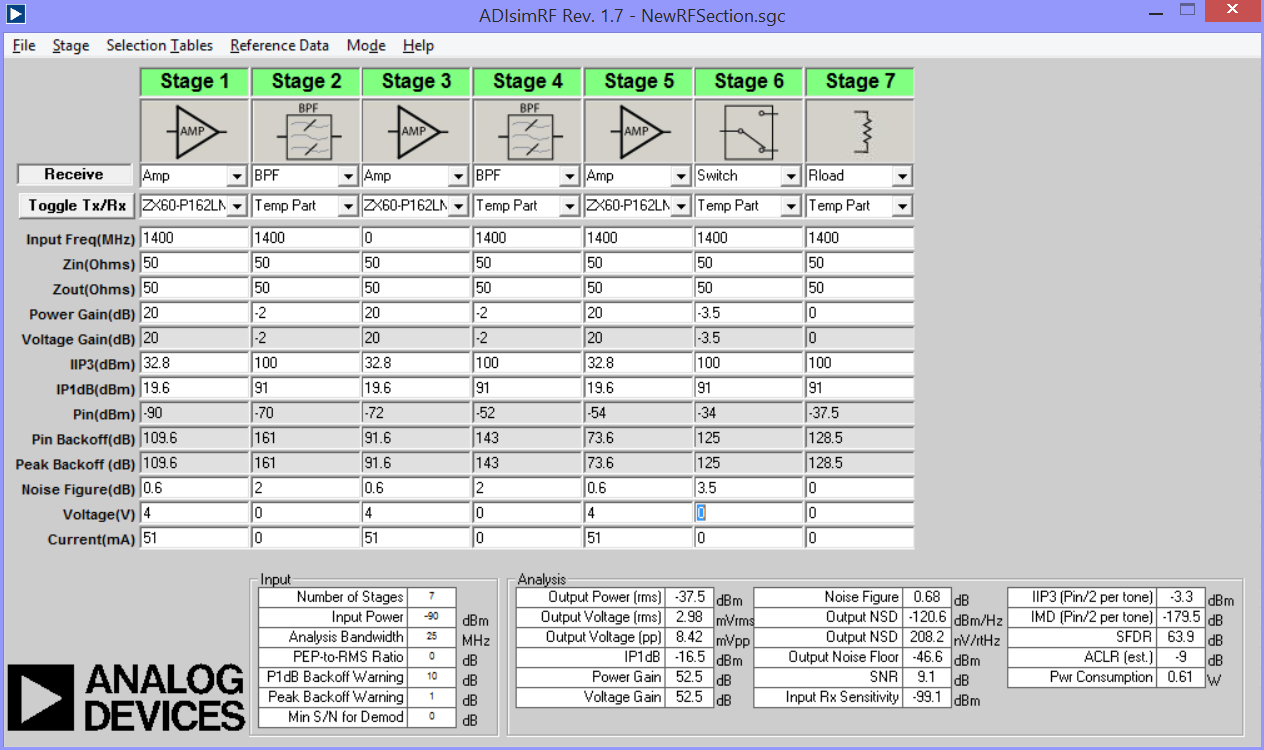
\includegraphics[width=0.8\linewidth]{Images/RF_Front_end.png}
%\isucaption{The ADISIMRF program used to verify the design of the RF Front End}
%\label{ISU_Rad}
%\end{figure}
%}

A typical RF front end uses a 3 stage Low Noise Amplifier (LNA) to amplifier the noise while keeping the noise contributed to the system as low as possible.  As with any radiometer, the first LNA is the most critical as it contributes the most to the overall system noise temperature.  For this reason a LNA that did not have a large gain but had a low noise figure is chosen. The second and third LNA has higher gain values at the cost of a higher noise figure, although not by much.  However, since they are further down the chain, they do not contribute as much to the total system noise.  

\begin{equation}\label{noise_factor}
F=F_1+\frac{F_2-1}{G_1}+\frac{F_3-1}{G_1 G_2}+\frac{F_4-1}{G_1 G_2 G_3}+\cdots +\frac{F_n-1}{G_1 G_2 G_3 \cdots G_{n-1}}
\end{equation}

Equation \ref{noise_factor} shows us how the noise factor and gain of the amplifiers affect each other.  It can be shown that the first amplifier or first noise figure in the system contributes the most to the overall system noise figure.  Additional components contribute, but at a much lower contribution.

\section{Mapping Traditional Radiometer Functions to a Software Defined Radio Radiometer}

In order to recreate a radiometer in software we need to identify the key components of a radiometer and then recreate those components in software.  As discussed in chapter three, the three components identified that are key to a radiometer is listed below.

\begin{enumerate}
\item Power detection
\item Integration
\item Bandwidth limitation or filtering
\end{enumerate}

The following sections will now examine how these items are mapped from their analog component to the software or digital component.

\subsection{Power detection}

Power detection is a key ability that allows a radiometer to function.  At its core a radiometer is a power detector.  Therefore, the implementation of power detection is a crucial function of a software defined radio radiometer.

A traditional radiometer uses a square-law detector which takes the input signal and produces a voltage that is proportional to the square of the voltage.  This allows us to take an analog RF signal and convert the noise voltage that for all intense and purposes has a mean value of zero, and produce a noise power.

{\begin{figure}[h!tb] 
\centering
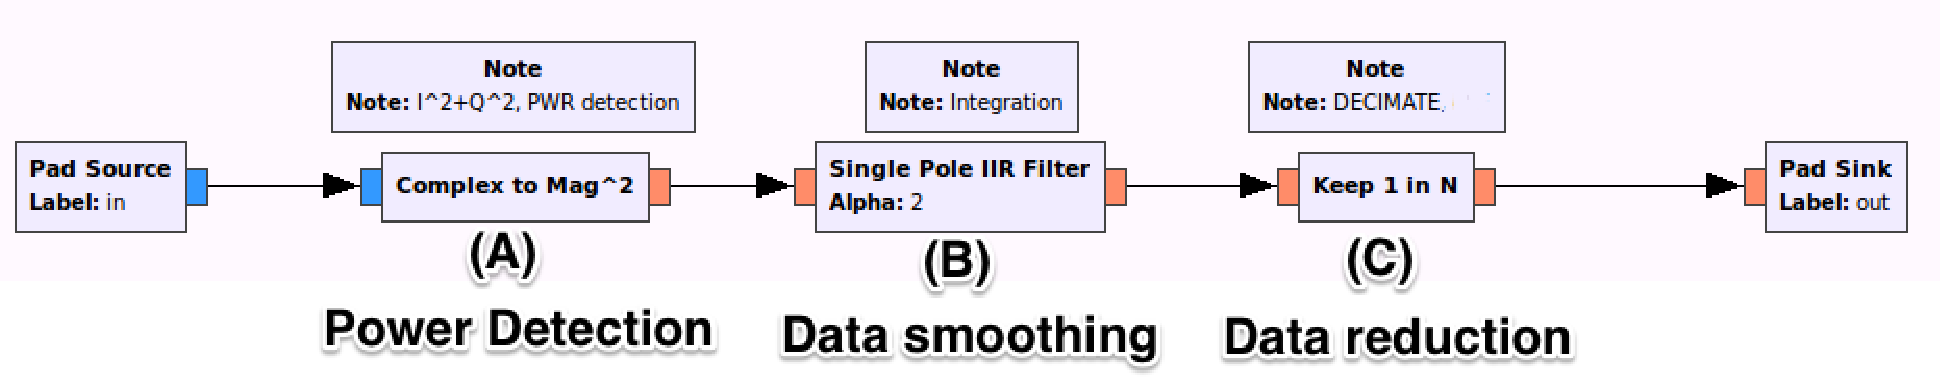
\includegraphics[width=17cm]{Images/TPR_grc.png}
\isucaption{A block diagram showing how the radiometer performs the equivalent square law detector in software.}
\label{square_block}
\end{figure}
}

To implement this in software we need to build a square law detector mathematically.   A square law detector mathematically is the sum of the squares.  Once the signal has been digitized, it is expressed in data bits of I and Q, which represent in-phase and quadrature-phase of the signal.  By squaring each term, we get the desired result of the power of the signal [\cite{Sarijari}][\cite{Rashid}] can be shown in equation \ref{sdr_x2}.

\begin{equation}\label{sdr_x2}
I^2+Q^2 = P_{out}
\end{equation}

Therefore, like the analog square-law detector we are taking peak voltage values, which has an equivalent noise voltage and a mean value of zero, and square them to produce a noise power that is proportional to the square of this amplitude.  Figure \ref{square_block} shows the GNURadio blocks used to perform this function.

Like the analog square-law detector, this signal will fluctuate rapidly and to improve the sensitivity of the radiometer we wish to integrate this signal.  We now want to look at how we can replicate a RC filter or integrator in the software defined radio.

\section{Integration}

Another step that we typically do in a traditional radiometer is to integrate the signal over time.  This gives us an average of the signal and smooths out the output.  This also helps to improve the sensitivity of the radiometer by equation \ref{NEAT_EQ}.

In a traditional radiometer, we can integrate by using a simple integrator circuit, which consists of an op-amp, resistor and capacitor.  This circuit configuration is also equivalent to a low pass filter circuit as well, and the two are interchangeable.  We can then look at how we filter in the digital domain, and this is down with an infinite impulse response filter or IIR.  We can use this digital filter to then integrate the signal for our total power radiometer.

To begin, we will examine how a RC filter is analogous to an integrator where the R and C values determine our time constant and our integration time for the filter[\cite{Aitken}].  We know a RC filter is analogous to an integrator by looking at equation \ref{eq:rc_int}.  A SDR however operates in the digital domain at discrete intervals.  One type of filter that can be used is the Infinite Impulse Response (IIR) filter. 

\begin{equation}\label{eq:rc_int}
\frac{1}{RC}\int{V_idt}
\end{equation}


To begin with, we look at what an analog RC filter looks like. 

{\begin{figure}[h!tb] 
\centering
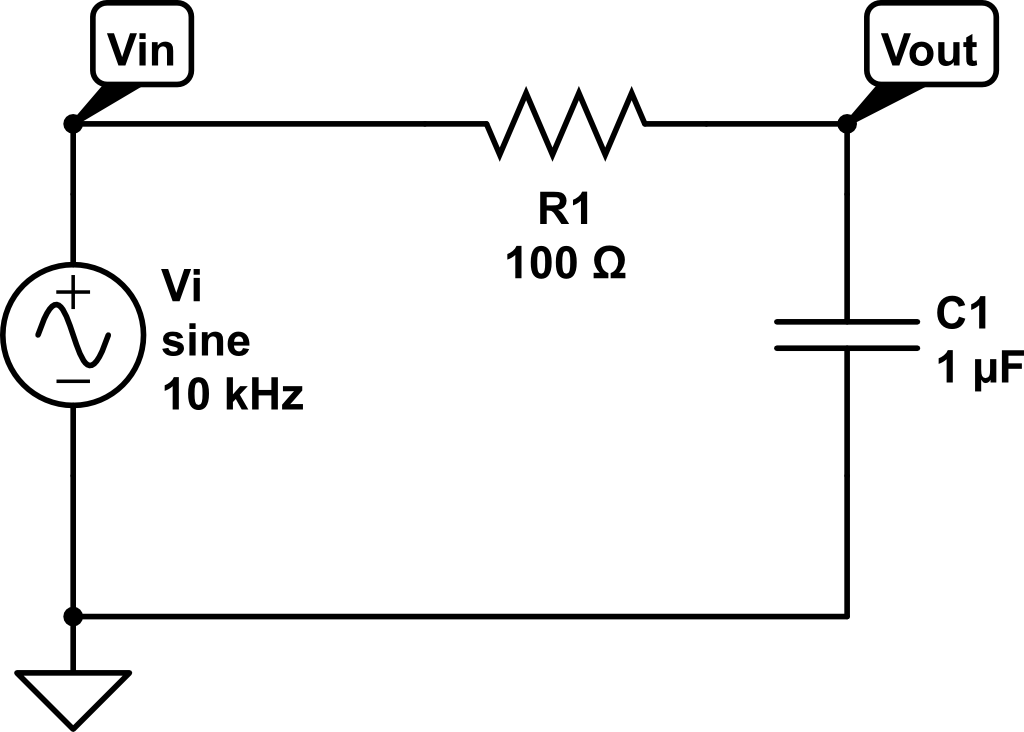
\includegraphics[width=10cm]{Images/rc-circuit.png}
\isucaption{A simple RC circuit}
\label{rc_circuit}
\end{figure}
}

This circuit can be represented by equation \ref{eq:rc_circuit_eq}.

\begin{equation}\label{eq:rc_circuit_eq}
\frac{V_{in}-V_{out}}{R}=C\frac{dV_{out}}{dt}
\end{equation}

A Finite Impulse Response (FIR) filter is a digital filter that can take an impulse signal and decays to zero after a finite number of iterations.  This type of digital filter can be represented by equation \ref{FIR_Eq} which mathematically expresses the FIR Filter.

\begin{equation}\label{FIR_Eq}
y_n=\displaystyle\sum\limits_{i=o}^{P-1} c_ix_{n-i}
\end{equation}

This simply says that the nth output is a weighted average of the most recent P inputs.  

An Infinite Impulse Response (IIR) filter is the same as the FIR filter, except that we add a summation term which feeds back the previous output.

\begin{equation}\label{IIR_eq}
y_n=\displaystyle\sum\limits_{i=o}^{P-1} c_ix_{n-i}+\displaystyle\sum\limits_{j=1}^{Q} d_jy_{n-j}
\end{equation}

Equation \ref{IIR_eq} shows that a FIR filter is a IIR filter, except that $Q=0$[\cite{Cross}].  

To get a better understanding on how the digital IIR filter relates to the RC filter analog, we can look at the Fourier Transform and the relationship of the input to the output in the frequency domain.

\begin{equation}\label{Fourier_IIR}
H(f)=\frac{\displaystyle\sum\limits_{j=o}^{P-1} c_je^{-2\pi ijfT}}{1-\displaystyle\sum\limits_{k=1}^{Q} d_ke^{-2\pi ikfT}}
\end{equation}

In equation \ref{Fourier_IIR}, $f$ is our frequency in Hz and $T$ is the time between samples in seconds and is related to our sampling frequency.

We now want to show the link between our analog RC circuit and the IIR filter.  Looking at equation \ref{eq:rc_circuit_eq}, which represents the differential equation relating the input voltage $V_{in}$ to the output voltage $V_{out}$, we can substitute for input and output of our IIR filter.  Since we are now in the time domain, we need to define what $T$ is and we can do that using equation \ref{sampling_rate_eq}.

\begin{equation}\label{sampling_rate_eq}
T=time between samples=\frac{1}{sampling rate}
\end{equation}

We can now relate our input voltage to the input to our IIR filter and the output voltage to the output of our IIR filter.

\begin{equation}\label{input_IIR}
x_n=v_{in}(nT)
\end{equation}

\begin{equation}\label{output_IIR}
y_n=v_{out}(nT)
\end{equation}

We can now rewrite our difference equation with $x_n$ and $y_n$.

\begin{equation}\label{diff_xn_yn}
\frac{x_n-y_n}{R}=C\frac{y_n-y_{n-1}}{T}
\end{equation}

Finally, we can solve for $y_n$ which results in our final equation for showing how a IIR filter is related to an RC filter.

\begin{equation}\label{final_IIR_RC}
y_n=\frac{T}{T+RC}x_n+\frac{RC}{T+RC}y_{n-1}
\end{equation}

It can be seen that an IIR filter can have the same frequency response as we expect from an analog RC filter.  As our sampling rate approaches infinity, the approximation gets closer to the original response from the analog RC circuit.  

For the cutoff frequency of a RC circuit, we know that it has the relationship shown in equation \ref{RC_relationship}.

\begin{equation}\label{RC_relationship}
f_c=\frac{\sqrt{3}}{2\pi RC}\rightarrow RC=\frac{\sqrt{3}}{2\pi f_c}
\end{equation}

The $RC$ term gives us our time constant of the circuit and can be used to calculate out our coefficients.  We are not concerned about the actual values of R and C with our IIR filter, instead we just need the product of R and C.  

In GNURadio most of the work is done for us.  We can simply enter in our desired cutoff frequency and GNURadio will calculate our IIR filter coefficients.  However, this shows that an IIR filter works much like an analog RC low pass filter.

\section{System overview}

Like a traditional radiometer, the SDR will use an antenna to look at the target of interest.  SDRs still use a RF stage that takes the power from the source and amplifies it.  The difference though begins after that.  A SDR will then sample and generate I and Q values that represents the amplitude and phase of the signal.  From there, this data is sent to a computer to be processed.  We can then use this information to calculate the power that is being seen.  In addition, we can manipulate the signal in other ways such as applying a filter to filter out an unwanted source.

As we have shown the two of the major components of a traditional radiometer, the power detection and integration of the signal can be replicated in software and therefore can be implemented in a software defined radio.  The information can now be stored, displayed or both for further analysis.  

There is one component of the software defined radio that we are not able to implement in software and that is with the signal amplification.  This however does play a major role in the performance of the radiometer and is a key element that should not be overlooked.  While this is not implemented in software, it still plays a critical role in our software defined radio radiometer. 

Next we will look at the software used in defining the radiometer.  It will also be shown what the impact is of this software on the performance of the radiometer.

\subsection{Control of the SDR Hardware through GNURadio}
The N200 sends all data across the 1 Gbps connection to be read in by a host computer running GNURadio.  This data is the raw I/Q values that is read by the on board A/D and processed by the on board FPGA.  An example of a very simple GNURadio software implementation would simply take this data and store the data to a hard drive in a file.  This can be very handy if we want to simply record the data and then process it later.  However, depending on the sample rate, it can consume a large amount of storage.  A short recording can easily consume 1-2 GB with a sample rate of 10 Msps.  It also does not give us any immediate feedback on the radiometer and it does not give us controls of the radiometer such as frequency, integration time or other key variables.  Fortunately GNURadio has tools that allows us to build up a very rich application that is able to give us the data we need and control the software defined radio as well.

The GNURadio Companion allows us to create python code that is used to not only receive the data from the SDR but also perform signal processing on the incoming information.  Additional controls are added that allow for tuning of the signal processing parameters and control of the radio functions.  This allows us to build up an application that can be run on any computer that is capable of running GNURadio.  

{\begin{figure}[h!tb] 
\centering
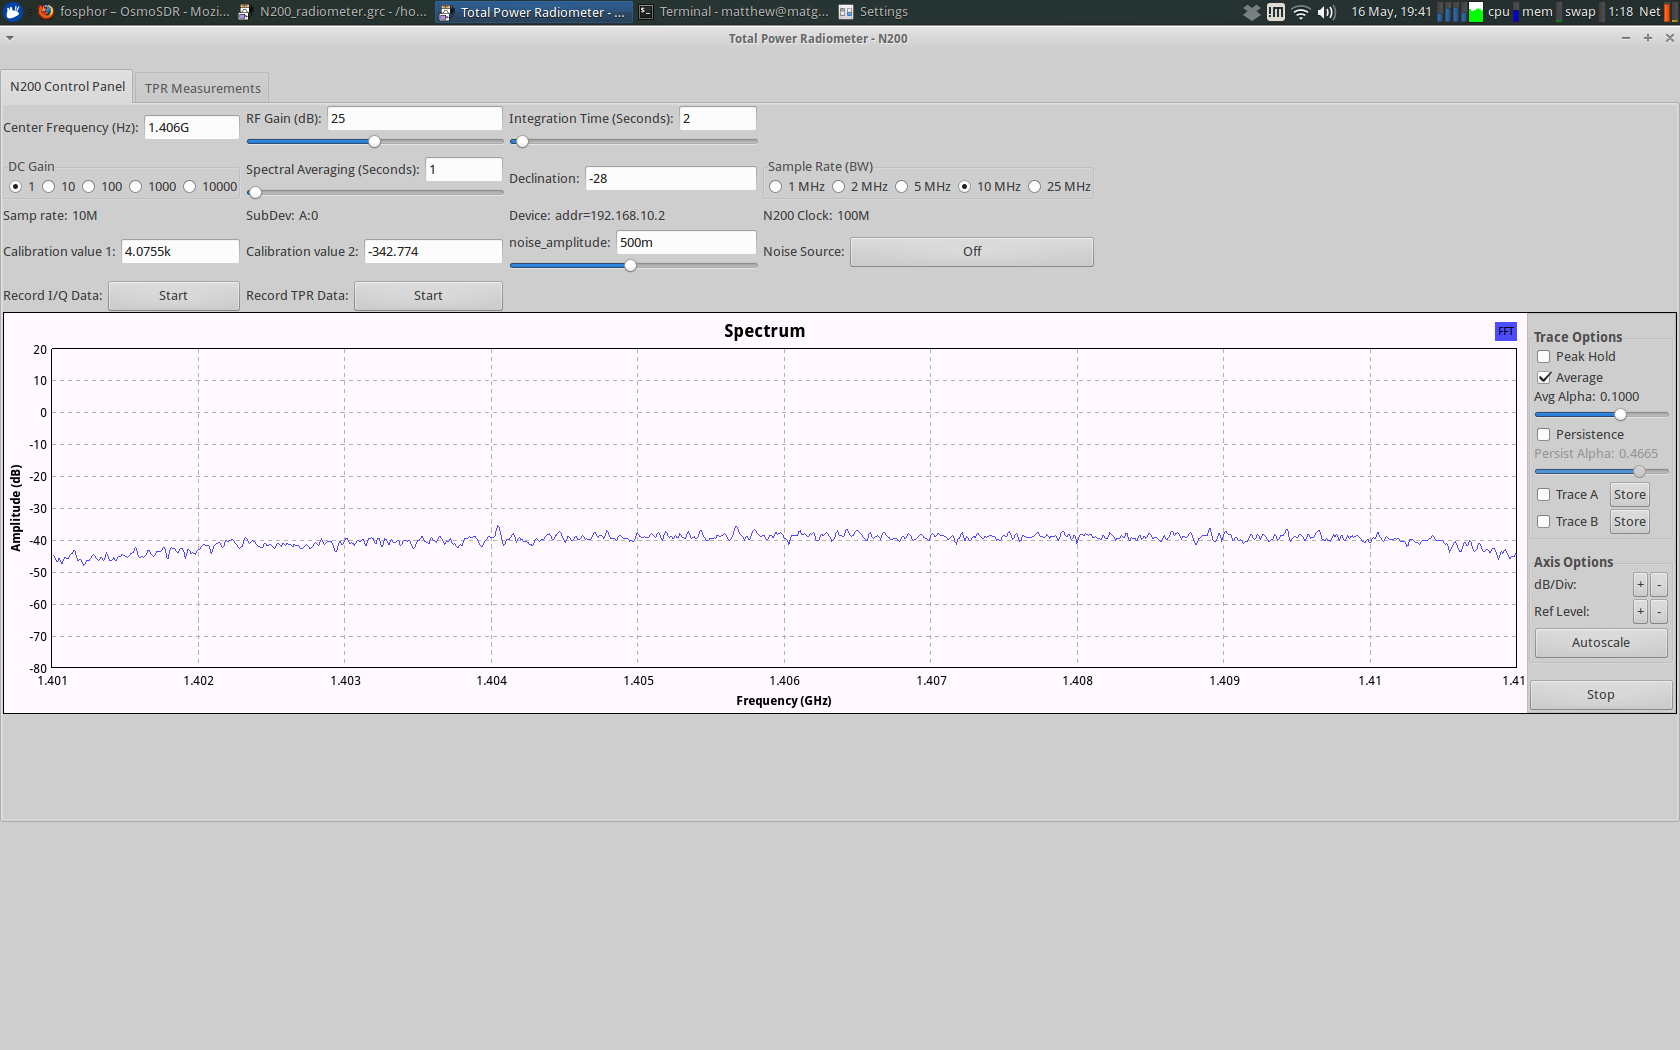
\includegraphics[width=17cm]{Images/radiometer_gui.png}
\isucaption{A screenshot of the interface made for communication with and controlling the software defined radio}
\label{radiometer_gui}
\end{figure}
}

Through this interface we are able to control several key aspects of not only the radio hardware within the SDR but also with the behavior of the radiometer as well.  Hardware control of the SDR hardware allows us to change frequency and also adjust gain values within the N200.  Bandwidth is another parameter that can be altered from here as well.  Bandwidth affects the bandwidth for the RF signal, but also has an impact on the radiometer sensitivity as well.  Additional controls allows for alterations to the radiometer and includes being able to adjust the integration time of the radiometer.  

\subsection{Impact of the Controls Related to Radiometry}

The controls that have been added for controlling the radiometer can have a large impact on the performance of the radiometer.  There is a reason why these controls were added to the GUI for the radiometer and that is they play key roles in how the radiometer performs.  

For any radiometer noise temperature is a large consideration and is critical to the design of the radiometer.  One method to determine how well a radiometer is to look at the sensitivity of the radiometer.  We can do this by looking at the smallest change in temperature the radiometer can see.  We will call this the Noise Equivalent $\Delta T$ or $NE\Delta T$ of the radiometer.  The equation for this is shown below.

\begin{equation}
NE\Delta T=\frac{T_{A}+T_{sys}}{\sqrt{\beta * \tau}}
\end{equation}

$\beta$ can be changed by changing the sample rate of the SDR.  The sample rate effectively controls the bandwidth in which the SDR is operating at.  This also gives us a band-pass filter as well, since the SDR will not respond to frequencies outside of this bandwidth.  

$\tau$ is the integration time for the radiometer.  This parameter is set by the user through the GUI and allows us to change the integration time in seconds.

\subsection{GNURadio Data Handling}
Once we have the data that has been processed by the software defined radio we will want to display this information and be able to store the data so we can analyze it later if needed.  Data display can be handled GNURadio where we can plot the total power over time.  This allows the user to be able to visualize the total power and be able to determine if the total power has increased or decreased over the time window shown.  

Although not usually needed for a total power radiometer we also have the ability to look at the signal in terms of a frequency versus amplitude.  This allows looking for any unusual signals that may be interfering with the system or causing erroneous data with our radiometer.  

Finally, we will want to store the data so we can do additional analyses on it at a later time.  The GNURadio program allows us to store the data in two formats.  The first format is storing the raw I/Q data from the radiometer.  This format allows us to playback the data through GNURadio at a later time.  This can be useful for if we wish to change parameters in GNURadio such as bandwidth or integration time.  It is also a good diagnostic tool as we can check that the signal coming in is clean or if we need to apply additional filters to remove an unwanted signal. This file may be quite large, consuming several gigabytes of data for a 20 MHz wide signal in a matter of minutes of record time.

The second format is the total power that has been calculated by the radiometer.  This file is much smaller since much of the signal information has now been reduced to simple power versus time information.  This allows for easy manipulation through any math program such as Matlab for analysis.  

\subsection{GNURadio Data Display}
The information from the software defined radio can be displayed through GNURadio to show a number of things.  Since we have both frequency and magnitude information we can display this information.  We are able to also display the information that shows the total power that is being seen by the radiometer as well.

{\begin{figure}[h!tb] 
\centering
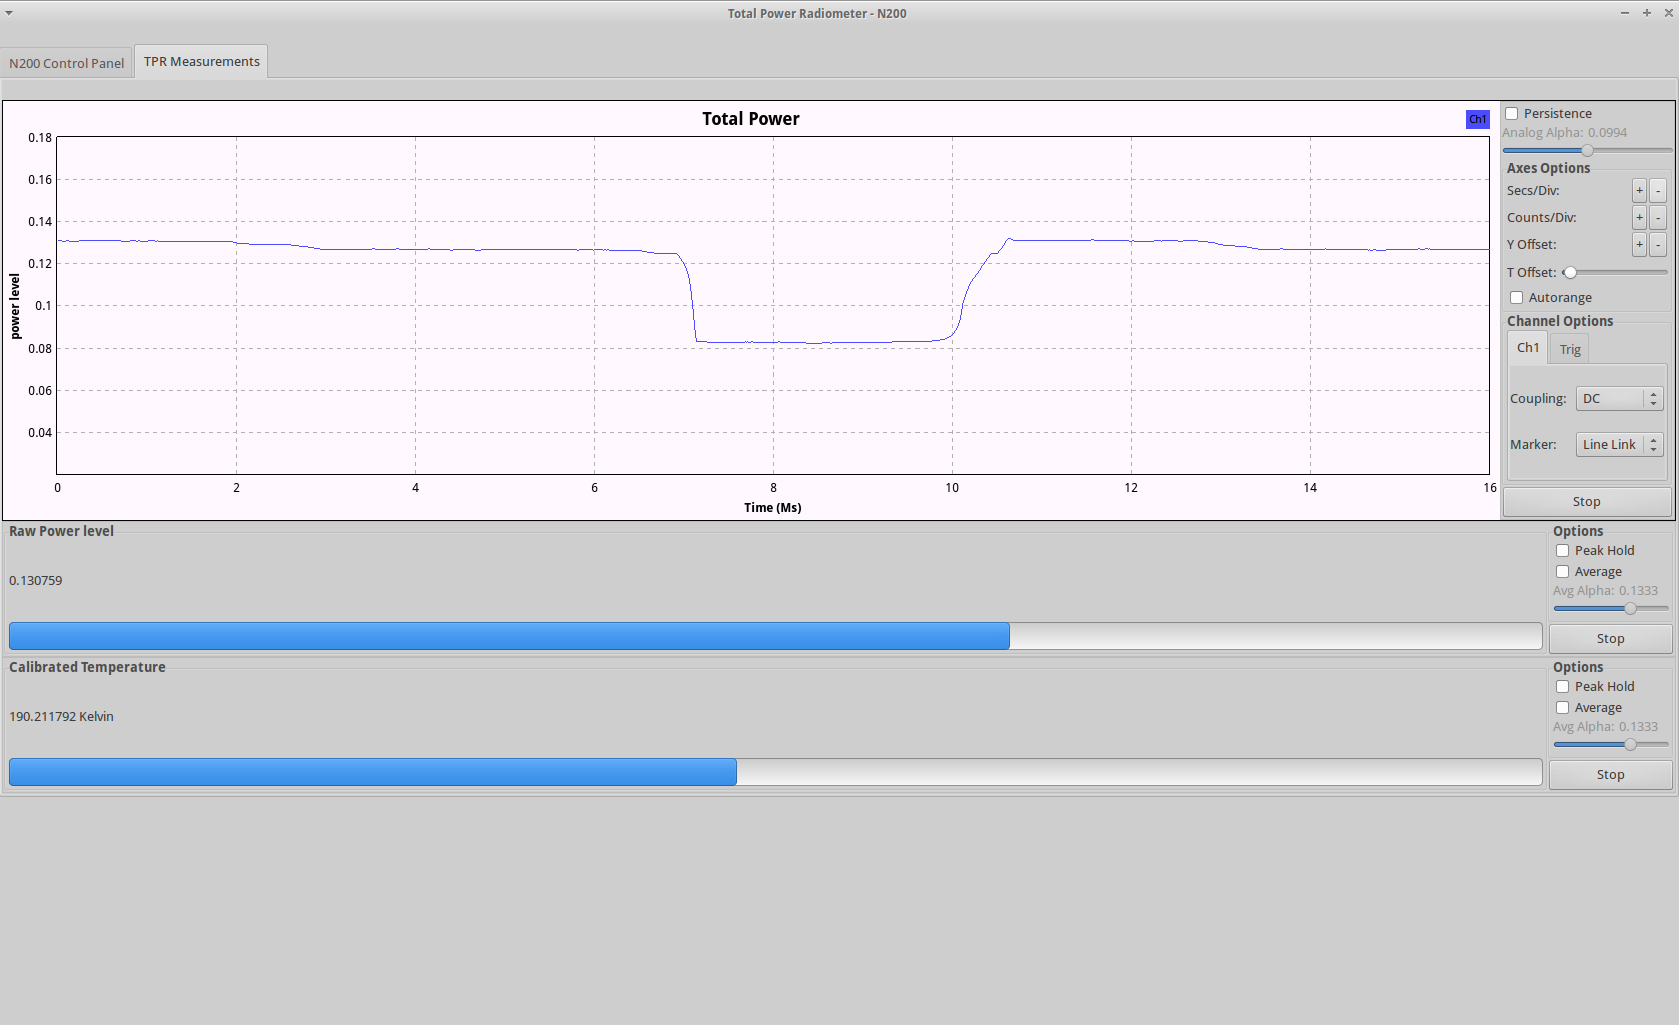
\includegraphics[width=17cm]{Images/Lab1_TPR_at_end_exp.png}
\isucaption{A screenshot showing the ticker tape display for the total power readings.  In addition, raw and calibrated noise temperature is shown below.}
\label{radiometer_tpr_display}
\end{figure}
}

We are not limited to just total power from the radiometer.  If the radiometer has been calibrated, those calibration points can be entered and GNURadio can calculate the calibrated noise temperature.  Additional information may also be added as needed.  For example, we are able to view the full spectrum that the radiometer sees.  This can be a useful tool for looking at potential RFI issues.  
%----------------------------------------------------------------------------------
%Everything below this needs to be moved/shifted or deleted

%\section{Square-law Detector Performance}
%The Square-law detector was added to our system in order to give us another reference point and to help verify the power output that the software defined radio.  Performance of our square-law detector is based on two items; the sensitivity of the diode used in the square-law detector and the analog to digital converter used to convert the analog voltage to a digital value.  The sensitivity of this device accounts for most of the performance factor of the system.  In our system the output of this square-law detector is then feed directly into an analog to digital converter.  Therefore, the performance of this A/D converter needs to be accounted for as well [\cite{Terlep}].  

%For our square-law detector, it has a noise output of $25nV/ \sqrt{Hz}$ at 100 kHz and will detect a signal as low as $-60$ dBm.  This works will with our needs since the RF front end brings the noise floor to approximately $-30$ dBm.
